\begin{figure}
    \centering
    \resizebox{0.48\textwidth}{!}{% Scale to half the page width
    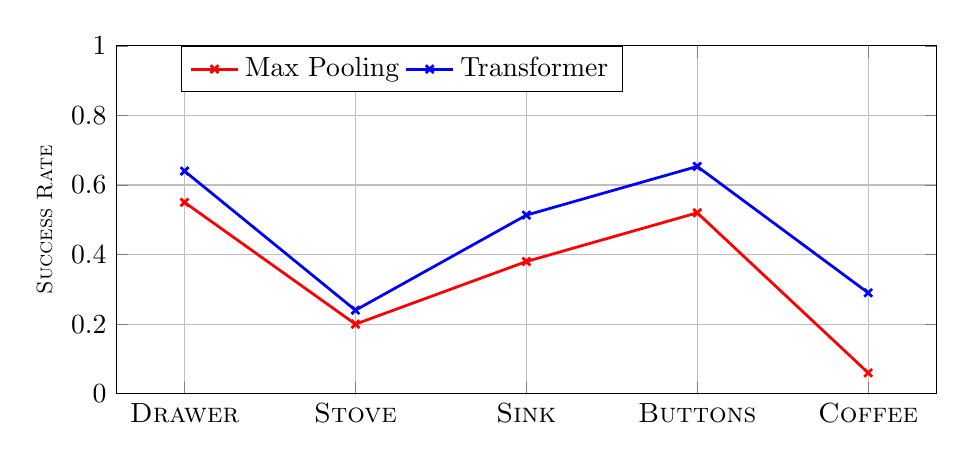
\begin{tikzpicture}[baseline]
    \definecolor{lightgray204}{RGB}{204,204,204}
    \definecolor{crimson}{RGB}{214,39,40}
    \definecolor{darkgray}{RGB}{176,176,176}
    \definecolor{darkorange}{RGB}{255,127,14}
    \definecolor{darkturquoise}{RGB}{23,190,207}
    \definecolor{forestgreen}{RGB}{44,160,44}
    \definecolor{goldenrod}{RGB}{188,189,34}
    \definecolor{gray}{RGB}{127,127,127}
    \definecolor{mediumpurple}{RGB}{148,103,189}
    \definecolor{orchid}{RGB}{227,119,194}
    \definecolor{sienna}{RGB}{140,86,75}
    \definecolor{steelblue}{RGB}{31,119,180}
    
    \begin{axis}[
        height=6cm,
        width=12cm,
        bar width=3.5pt,
        ylabel=Success Rate,
        ylabel style={
            font=\footnotesize\scshape
        },
        ymin=0, ymax=1,
        legend style={at={(0.348, 1)}, anchor=north, legend columns=-1},
        symbolic x coords={drawer, stove, sink, buttons, coffee},
        xtick=data,
        % Override the actual tick labels with capitalized names:
        xticklabels={Drawer,Stove,Sink,Buttons,Coffee},
        xticklabel style={font=\scshape},
        ymajorgrids,
        grid=both,
    ]
    
    % -- Max Pooling (red) --
    \addplot [
        draw=red,
        line width=1pt,
        mark=x,
        mark options={solid},
    ]
    coordinates {
        (drawer, 0.5500)
        (stove, 0.2000)
        (sink, 0.3800)
        (buttons, 0.5200)
        (coffee, 0.0600)
    };
    
    % -- Transformer (blue) --
    \addplot [
        draw=blue,
        line width=1pt,
        mark=x,
        mark options={solid},
    ]
    coordinates {
        (drawer, 0.6400)
        (stove, 0.2400)
        (sink, 0.5133)
        (buttons, 0.6533)
        (coffee, 0.2900)
    };
    
    \legend{Max Pooling, Transformer}
    \end{axis}
    
    \end{tikzpicture}
    }
    \caption{Success rates using max pool or transformer to obtain global feature vector of RGB images to use in AdaLN conditioning.}
    \label{fig:ablation_cond_vec}
\end{figure}
